\chapter{Nutzung des Backends}
\label{chapter:use}
  
  \section{Einleitung}
  \label{section:backend_introduction}
  
  Über \textbf{bwolf.de/backend} kann das Backend des BWolf-Systems erreicht werden.
  
  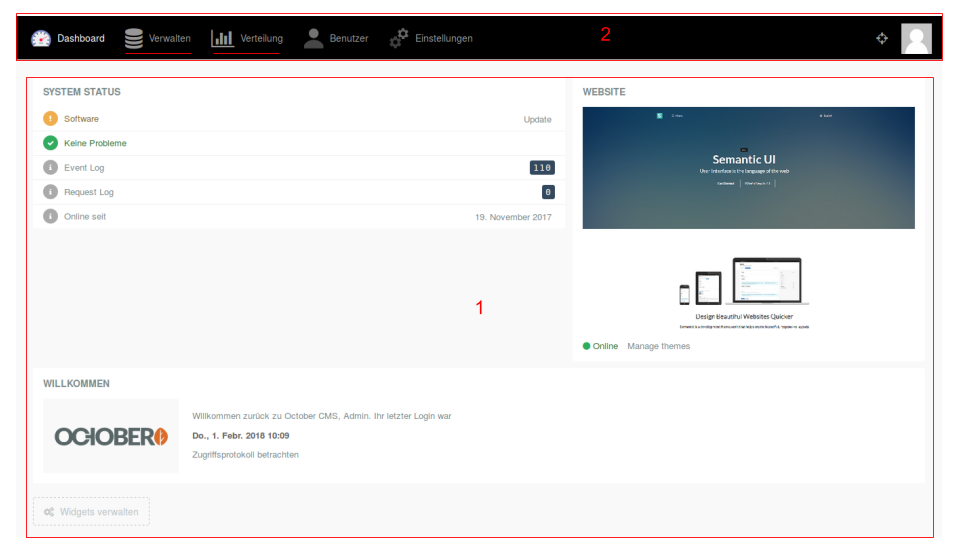
\includegraphics[scale=0.3]{backend/img/dashboard.png}
<<<<<<< HEAD
  \caption{\newline Der Begrüßungsbildschirm: Das Dashboard aus Sicht des Super-Admins.\newline
	  Normale Administratoren sehen in der oberen Navigation nicht den Punkt Benutzer}
=======
  %\caption{\newline Der Begrüßungsbildschirm: Das Dashboard aus Sicht des Super-Admins.
%      \newline Normale Administratoren sehen in der oberen Navigation nicht den Punkt ''Benutzer''}
>>>>>>> 299e46a733f53cc67ae936bd3d4070899f232aa0
  \begin{enumerate}
   \item Nach der Anmeldung begrüßt das \textbf{Dashboard} den Nutzer. 
	  Hier befinden sich drei Widgets:\newline
	  Bei der Begrüßung befindet sich eine Übersicht über den Systemstatus.\newline
	  Für die elementare Nutzung des Backends, müssen hier keine weiteren Änderungen vorgenommen werden.\newline
	  Sollte in dem Systemstatus ein Problem auftauchen, sollte einer der Entwickler (siehe \url{http://bwolf.uni-jena.de/impressum}) 
	  kontaktiert werden.\newline
	  Das Widget \textbf{Website} zeigt an in welchem Theme die Webseite erscheint. Hier sollte auch nichts weiter verändert werden.
	  Ganz zu unterst gibt es noch einen Button \textbf{Widgets verwalten}. 
	  Dieser spielt hier auch keine weitere Rolle, da alle vorhandenen Widgets bereits in das Dashboard integriert wurden.
   \item Über die obere Navigationszeile gelangt der Nutzer zu allen wesentlichen Bereichen des Backends.
	 Zur operativen Benutzung benötigt werden die Bereiche \textbf{Verwalten} und \textbf{Verteilung}
   \item[] In der oberen Navigationszeile befindet sich ganz rechts die Möglichkeit des Abmeldens.
   \item[] Das Fadenkreuz daneben ermöglicht es, das Frontend mit den momentan vorgenommenen Einstellungen zu betrachten.
  \end{enumerate}

  
  \section{Verwalten}
  \label{section:manage}
  
    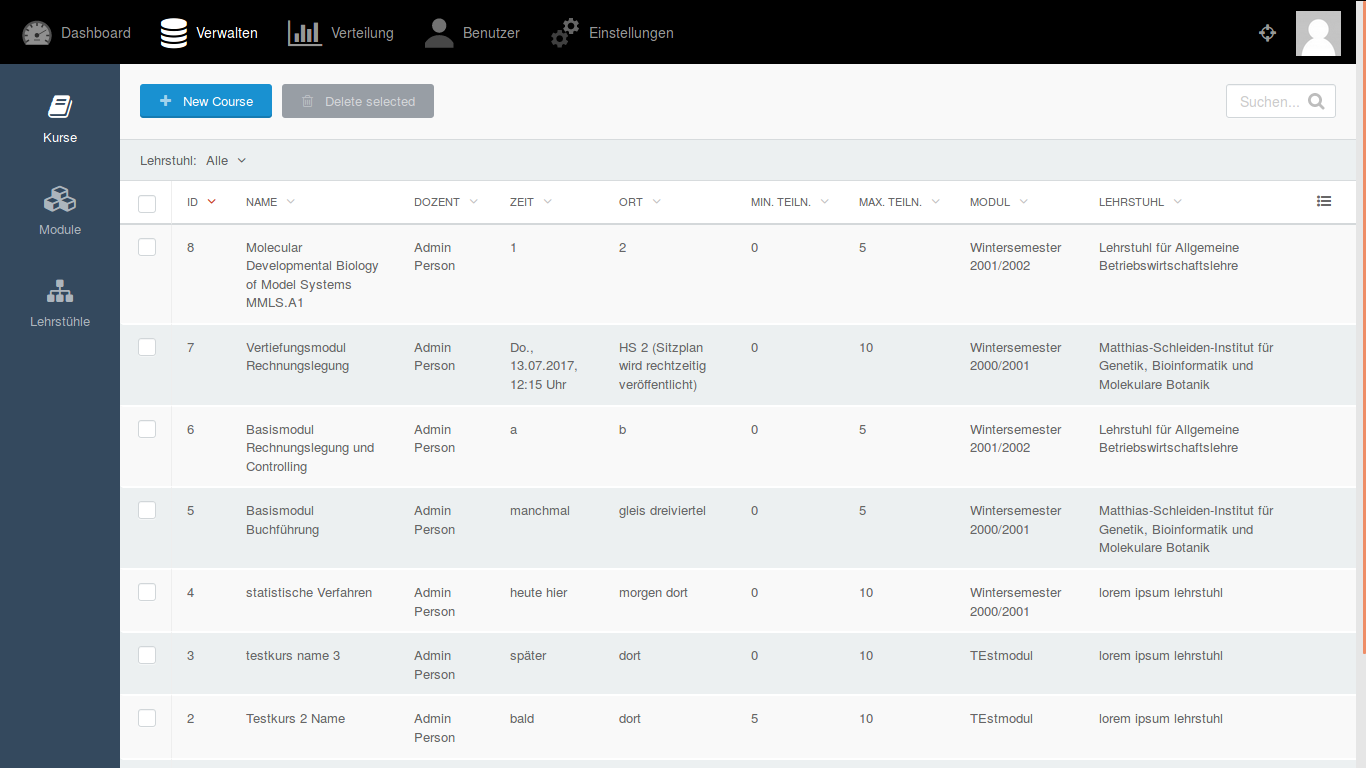
\includegraphics[scale=0.3]{backend/img/verwalten.png}

    In diesem Bereich können der Nutzer neue Module, Lehrstühle und Kurse anlegen.
    Anhand der linken Navigationsspalte können die entsprechenden drei Bereiche erreicht werden.

    In der Übersichtsliste der drei unterschiedlichen Bereiche Module, Lehrstühle und Kurse kann die Reihenfolge der Zeilenelemente durch Betätigen
    der kleinen Pfeile neben den Spaltennamen umsortiert werden.
    In der Kopfzeile dieser Übersichtsliste befindet sich ein Hamburger-Menü. 
    Wenn der Nutzer darauf klickt, öffnet sich ein Popup indem der Nutzer Spalten ein- oder abschalten kann.
    Darüber hinaus kann die maximale Anzahl an Zeileneinträgen pro Seite angegeben werden.
    
    \subsection{Module}
    
    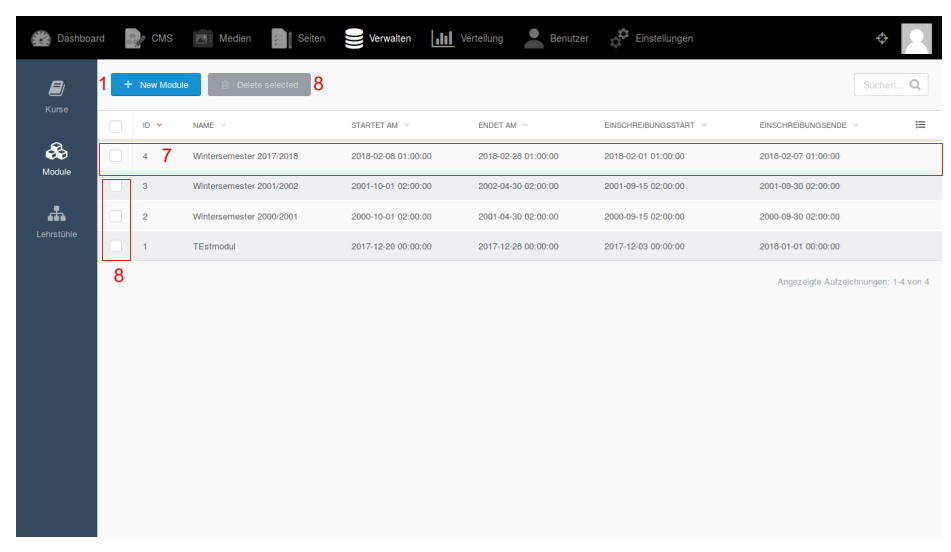
\includegraphics[scale=0.3]{backend/img/module_1.png}

    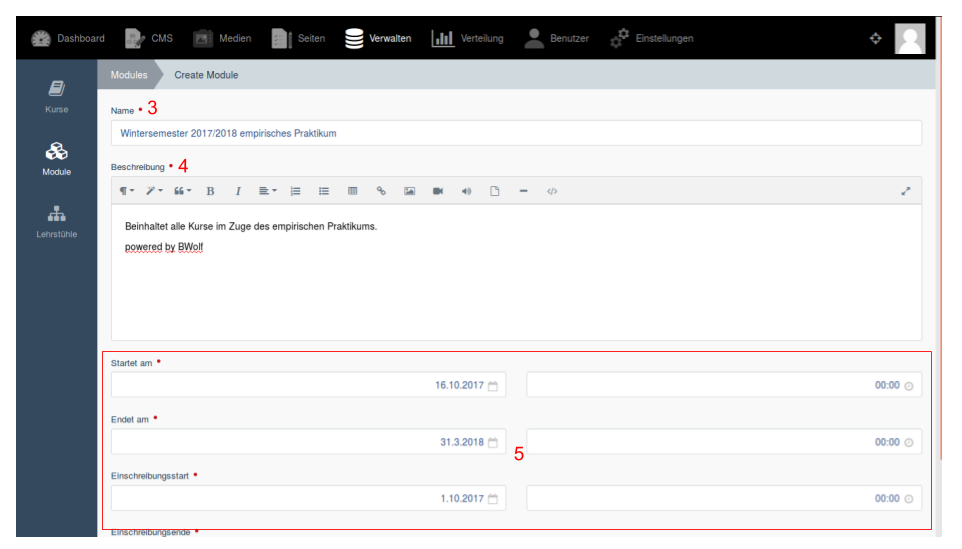
\includegraphics[scale=0.3]{backend/img/module_2.png}

    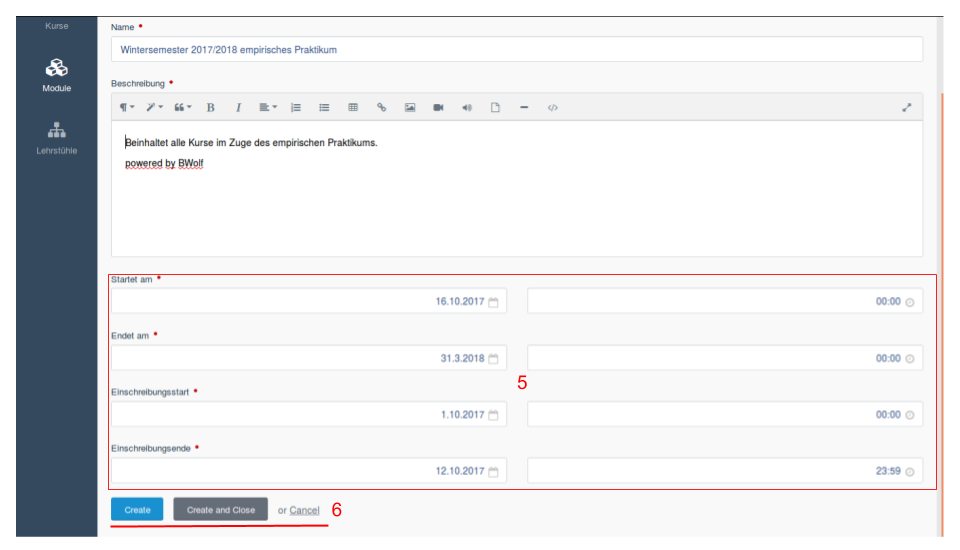
\includegraphics[scale=0.3]{backend/img/module_3.png}
    
    \begin{enumerate}
    \item Zuerst sollte ein neues Modul angelegt werden. Durch Betätigen des \textbf{+ New Module} - Buttons kann ein neuer Kurs angelegt werden.
    \item Hier müssen alle Pflichtfelder - gekennzeichnet durch einen kleinen roten Punkt neben der Feldbeschreibung - ausgefüllt werden.
    \item Ein möglicher Name für einen Modulnamen wäre beispielsweise \textit{Wintersemester 2017/2018 empirisches Praktikum}. Er beschreibt die Veranstaltung.
    \item In den Beschreibungstext können mützliche Informationen zu dem Modul angelegt werden.
	  Hier können neben einfachen Text auch Listen, Bilder, Tabellen und Medienelemente eingefügt werden.
    \item In den Datums- und Zeitfeldern wird der Zeitraum des Moduls angegeben, (beispielsweise \textit{16.10.2017, 00:00} bis \textit{31.03.2018, 23:59}) 
	  wie auch der Einschreibungszeitraum in denen sich Studenten für Kurse des Moduls einschreiben können (beispielsweise \textit{1.10.2017, 00:00} bis \textit{12.10.2017, 23:59}).
	  Um die Zeitdaten anzugeben, können die aufploppenden Kalender- und Uhrmenüs verwendet werden. Auch die Eingabe über Tastatur ist möglich.
	  Der Einschreibungszeitraum muss vor derm Starttermin des Moduls beginnen.
    \item Über \textbf{Create} wird das neue Modul angelegt. 
	  Durch Betätigen von \textbf{Create and Close} wird das Modul angelegt und der Nutzer landet zurück auf der Übersichtseite aller angelegten Module.
	  Mithilfe von \textbf{Cancel} wird der Erstellungsvorgang abgebrochen.
    \item Durch Anklicken eines der Module kann dieses erneut angepasst werden.
    \item Indem einige Module über die Auswahlkästchen am Beginn der Zeile ausgewählt werden, können diese dann über den Button \textbf{Ausgewählte löschen} entfernt werden.
    \end{enumerate}
    
    \subsection{Lehrstühle}
    
    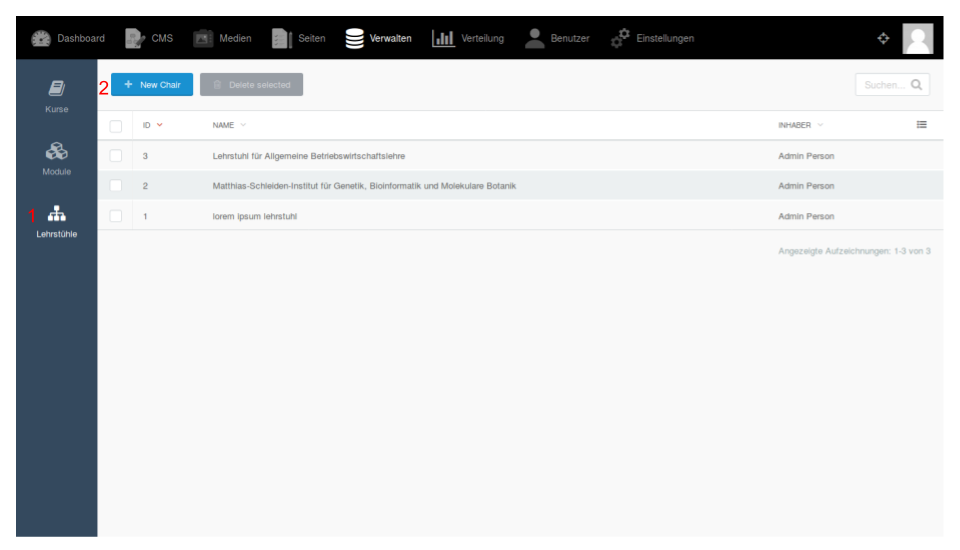
\includegraphics[scale=0.3]{backend/img/chairs_1.png}
    \begin{enumerate}
      \item Als nächstes sollten neue Lehrstühle hinzugefügt werden. Dies ist möglich über den dritten Punkt der linken vertikalen Navigation.
     \item Über \textbf{+ New Chair} kann ein neuer Lehrstuhl hinzugefügt werden. 
    \end{enumerate}

    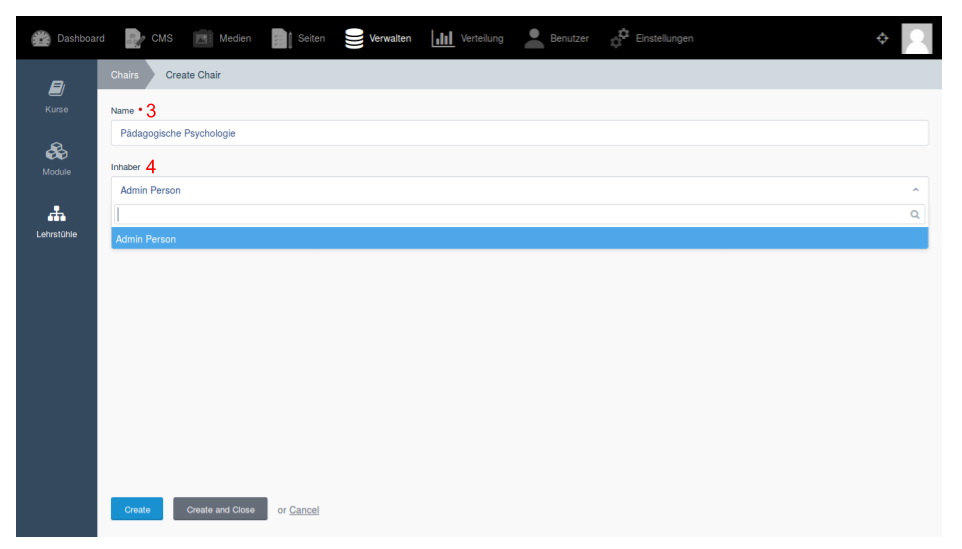
\includegraphics[scale=0.3]{backend/img/chairs_2.png}
    
    \begin{enumerate}
     \item[3.] Es muss ein Name vergeben werden. Namensgebung beliebig.
     \item[4.] Dem Stuhl kann nur ein Backend-Nutzer zugewiesen werden.
    \end{enumerate}

    \subsection{Kurse}
    
    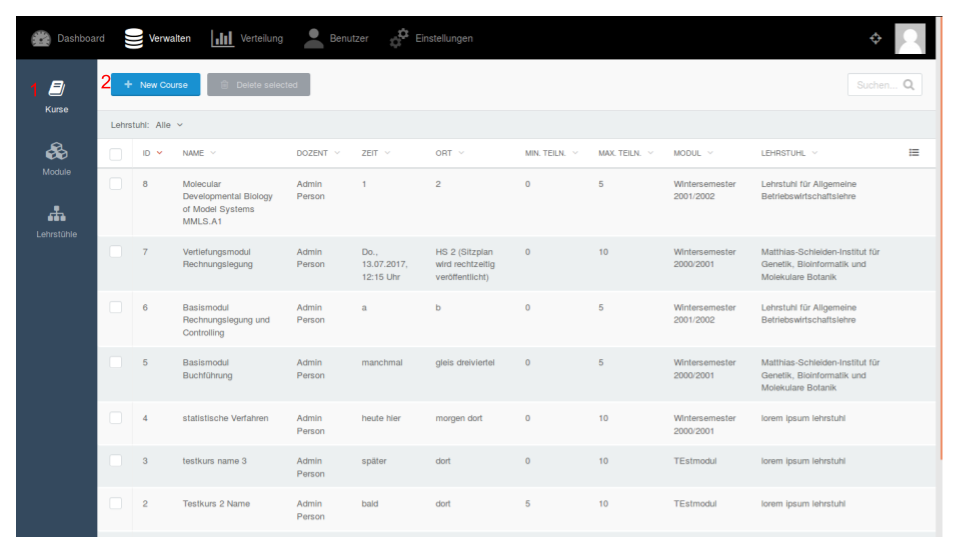
\includegraphics[scale=0.3]{backend/img/verwalten_kurse.png}
<<<<<<< HEAD
    \begin{enumerate}
     \item Über den ersten Punkt der linken Navigation kommt der Nutzer zur Kursübersicht.
     \item In der Kursübersicht kann der Nutzer über \textbf{+ New Course} einen neuen Kurs anlegen. 
    \end{enumerate}
    
=======
    %\caption{Verwalten in der Ansicht ''Kurs''}

>>>>>>> 299e46a733f53cc67ae936bd3d4070899f232aa0
    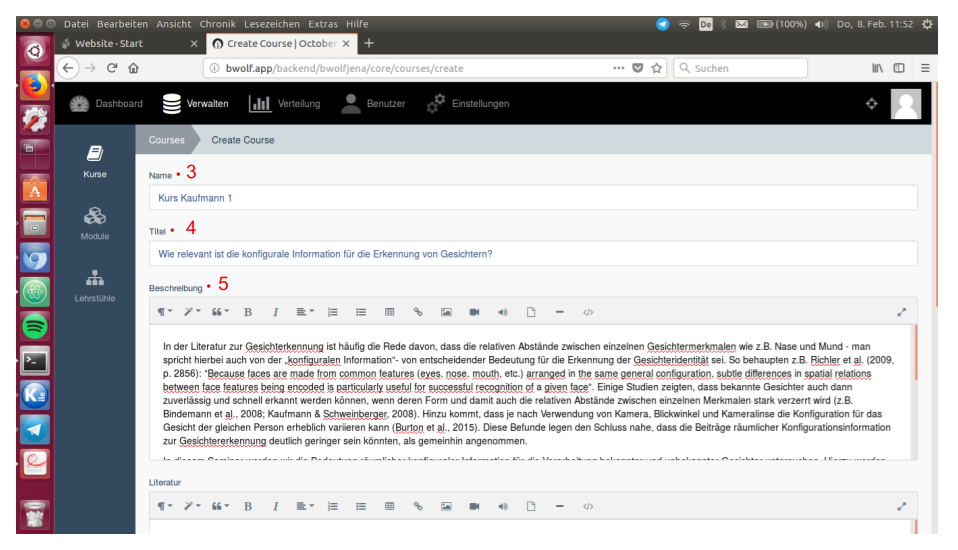
\includegraphics[scale=0.3]{backend/img/create_course_1.png}
    \begin{enumerate}
     \item[3.] Ein Kurs benötigt einen Kursnamen. Dieser Name kann zum Beispiel den Namen des Dozenten und evtl eine Zahl beinhalten. Zum Beispiel: \textit{Kurs Kaufmann 1}
     \item[4.] In dem Kurstitel sollte dann der eigtl Name des Kurses stehen. Beispielsweise \textit{Wie relevant ist die konfigurale Information für die Erkennung von Gesichtern?}
     \item[5.] Die Beschreibung dient als Hilfsmittel zur besseren Beschreibung des Kurses. Sie ist jedoch optional.
	       Hier können rich-text-Elemente wie Tabellen, Bilder und Textbearbeitung dafür genutzt werden.
    \end{enumerate}

    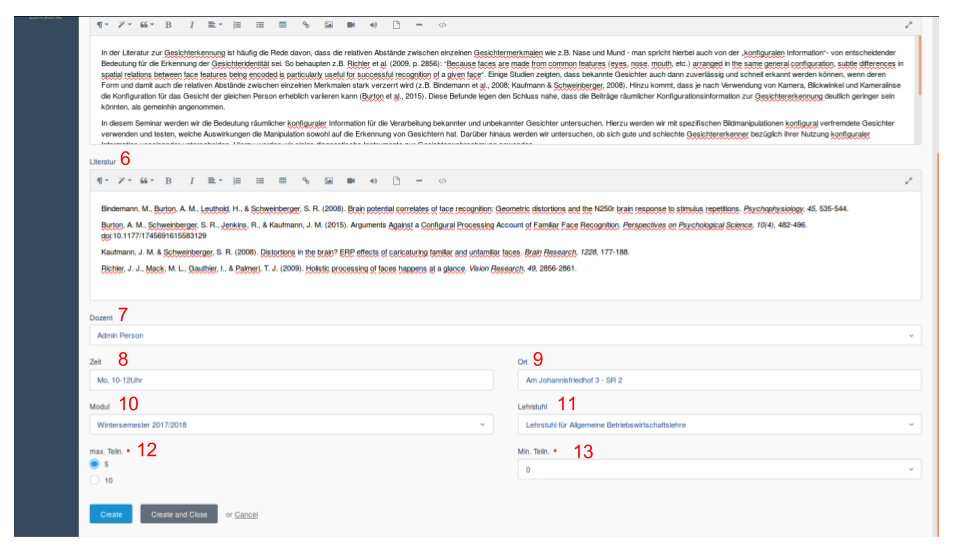
\includegraphics[scale=0.3]{backend/img/create_course_2.png}
    \begin{enumerate}
     \item[6.] Als gesonderten Bereich der Beschreibung gibt es die Literatur. Mithilfe einer Ungeordneten Liste kann hier Literatur eingetragen werden.
     \item[7.] Über Dozent kann dem Kurs ein verantwortlicher Dozent, bzw. Administrator zugewiesen werden.
     \item[8.] In der Zeiteingabe kann ein Text eingegeben werden. Zum Beispiel \textit{Mo, 10-12Uhr}. 
     \item[9.] Auch bei der Ortseingabe kann ein beliebiger Text eingegeben werden. \textit{Am Johannisfriedhof 3 - SR 2}
	       Ort und Zeitangabe sind nicht zwingend erforderlich.
     \item[10.]Über Modul kann der Nutzer den Kurs einem Modul zuordnen. Dies ist erforderlich, damit der Kurs in dem entsprechenden Modul auch angeboten werden kann.
     \item[11.]Auch sollte über Lehrstuhl dem Kurs ein Lehrstuhl zugeordnet werden. Dies ist nicht zwinged erforderlich.
     \item[12.]Nicht optional ist die Angabe, wieviele Teilnehmer der Kurs maximal haben darf. Hier kann zwischen fünf und zehn Teilnehmern gewählt werden.
     \item[13.]Ein weiteres Pflichtfeld ist die Angabe der minimalen Teilnehmerzahl. Sie kann erst angegeben werden, wenn eine maximale Teilnehmerzahl anegegeben wurde.
	       Dies ist wichtig, damit ermittelt werden kann, ob der Kurs zustande kommt oder nicht.
     \item[]Über die Buttons \textbf{Create} bzw. \textbf{Create and Close} kann der Kurs schließlich gespeichert werden. \textbf{Cancel} bricht den Erstellungsvorgang ab.
    \end{enumerate}

  
  \section{Verteilung}
  \label{section:distribution}
  
  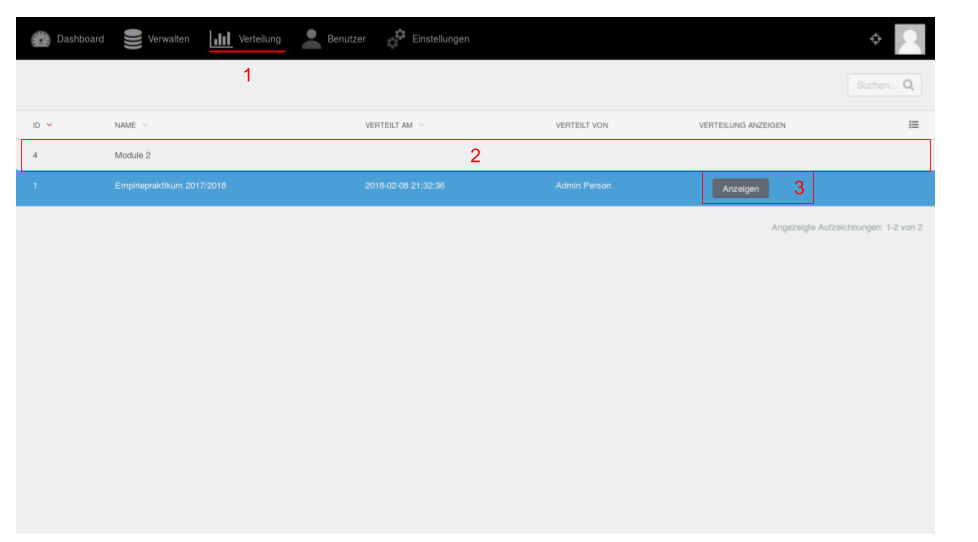
\includegraphics[scale=0.3]{backend/img/distribution_1 .png}
  
  \begin{enumerate}
<<<<<<< HEAD
   \item Um eine Verteilung berechnen zu lassen, wechselt der Nutzer in der oberen Hauptnavigation zu dem Punkt \textbf{Verteilung}.
=======
   \item Um eine Verteilung berechnen zu lassen, wechselt der Nutzer in der oberen Hauptnavigation zu dem Punkt ''\textbf{Verteilung}''.
>>>>>>> 299e46a733f53cc67ae936bd3d4070899f232aa0
   \item Indem der Nutzer auf eine der vorhandenen Module klickt, kann er mögliche Verteilungen der Studenten auf die Kurse generieren lassen.
	 Gegebenenfalls können keine Verteilungen generiert werden, zum Beispiel, wenn nicht genügend Kurse zum Verteilen vorhanden sind.
	 Sollte die Generierung erfolgreich gewesen sein, wird eine Übersicht der zur Verfügung stehenden Kurse geladen. 
	 (Siehe dazu die Punkte 4 bis 8)
   \item Wenn bereits von einem Backend-User für ein Modul mögliche Verteilungen berechnet wurden, kann über \textbf{Anzeigen} angezeigt werden, welcher Student welchen Kurs zugewiesen bekommen hat.
  \end{enumerate}
  
  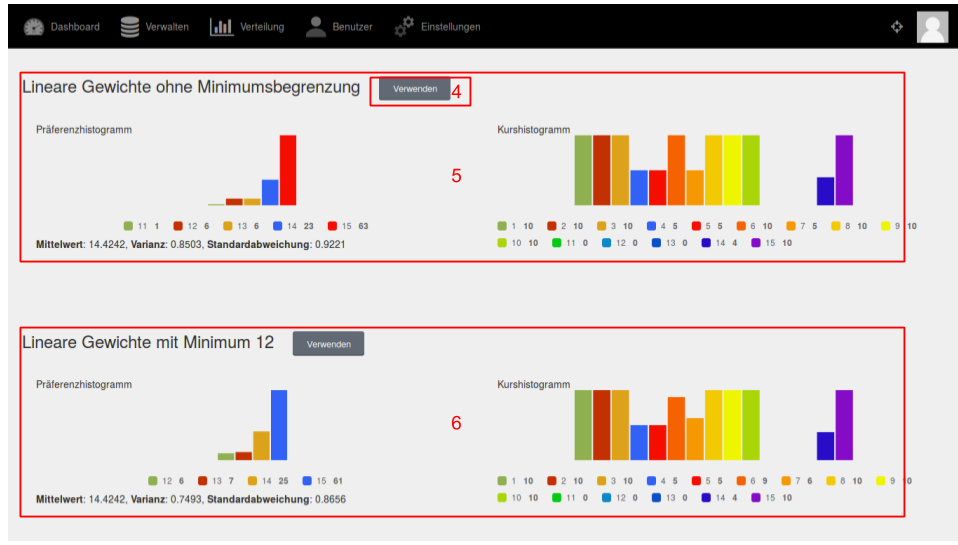
\includegraphics[scale=0.3]{backend/img/distribution_2.png}
  
  \begin{enumerate}
   \item[4.] Durch Betätigen einer der \textbf{Anwenden}-Buttons, öffnet sich ein kleiner Dialog, der abfragt, ob die ausgewählte Verteilung 
	    tatsächlich angewendet werden soll. Durch Bestätigung wird die entsprechende Verteilung auf die angemeldeten Studenten angewendet.  
   \item[5.] Als erstes betrachtet der Nutzer eine Verteilung mit linearen Gewichten ohne Minimierung
   \item[6.] Hier gibt es auch lineare Gewichte mit einer relativ hohen Minimierung (12). 
	     Erläuterungen zu den Verteilungen und dem Verteilungsalgorithmus an sich, siehe Kapitel~\ref{chapter:algorithm}. 
  \end{enumerate}

  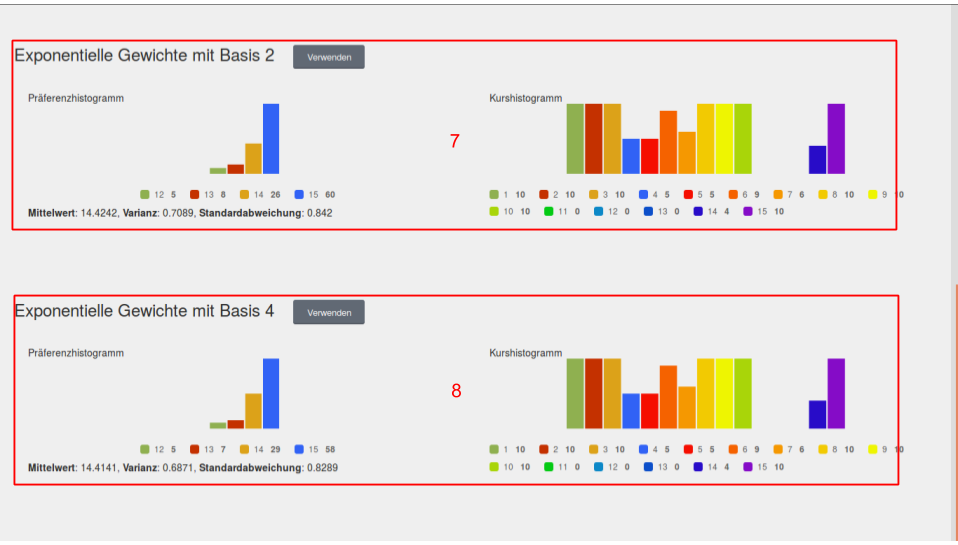
\includegraphics[scale=0.3]{backend/img/distribution_3 .png}
  \begin{enumerate}
   \item[7. und 8.] Neben linearen Gewichtsverteilungen hat der Nutzer auch die Möglichkeit exponentielle Gewichte zu verwenden
  \end{enumerate}

  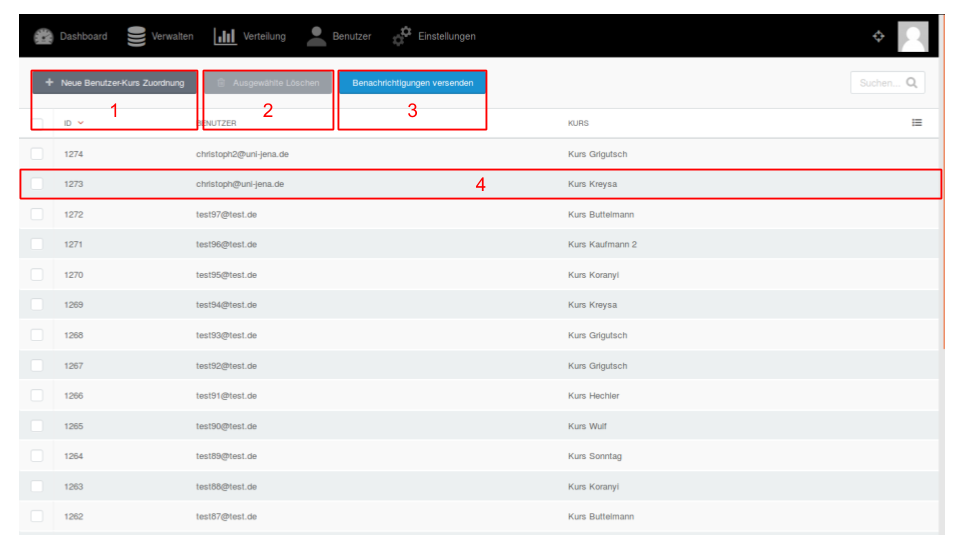
\includegraphics[scale=0.3]{backend/img/distribution_4.png}
  \begin{enumerate}
   \item Soll einem der Studenten einen anderem Kurs zugewiesen werden, kann dies durch den Button \textbf{+ Neue Benutzer-Kurs Zuordnung} erfolgen.
	 Dann gelangt der Nutzer auf die Seite mit dem hier drunter aufgeführten Bild (Erstelle Benutzer-Kurs Zuordnung).
   \item Wenn einer der eingetragenen Studenten aus der Liste entfernt werden, geschieht dies durch diesen Button \textbf{Ausgewählte Löschen}.
	 Dazu wird der entsprechende Student durch Klick in das weiße linke Feld seiner Zeile ausgewählt.
	 Dann ist dieser Button nicht mehr ausgegraut und kann benutzt werden.
   \item Wenn die Kursverteilugsliste fertig ist um veröffentlicht zu werden, 
	 können durch diesen Button \textbf{Benachrichtigungen versenden} die E-Mails an die Studenten versendet werden.
   \item Wenn eine der Zeilen ausgewählt wird, gelangt man in die entsprechende Ansicht, wie wenn man auf den Button \textbf{+ Neue Benutzer-Kurs Zuordnung} klickt.
	 Nur sind dann die entsprechenden Daten bereits in die Eingabefelder eingetragen. (Näheres dazu in dem Bild hier drunter.)
  \end{enumerate}

  
  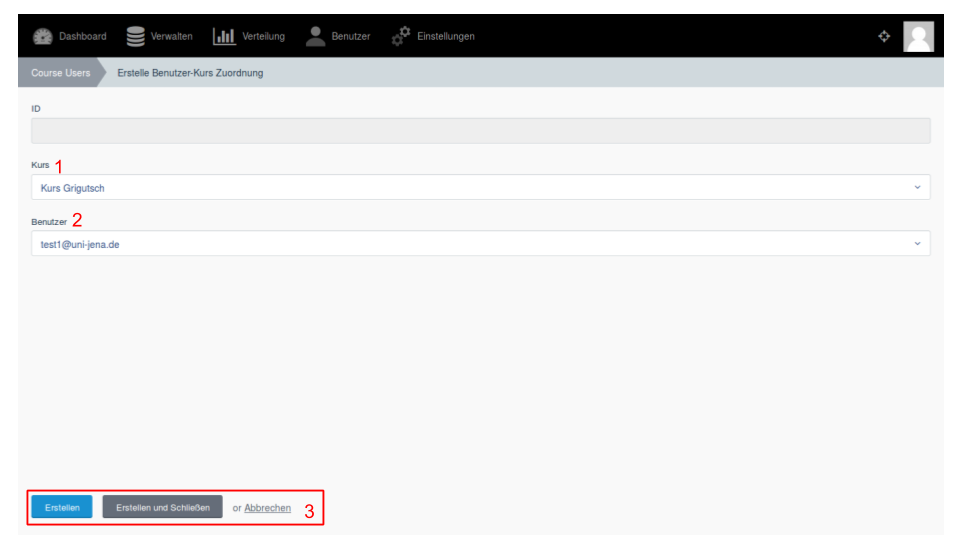
\includegraphics[scale=0.3]{backend/img/distribution_5.png}
  \begin{enumerate}
   \item Hier kann durch ein Dropdown-Menü ein entsprechender Student ausgewählt werden.
   \item Hier kann auf die selbe Art und Weise ein anderer Kurs ausgewählt werden.
   \item Durch einen der \textbf{Speichern}-Buttons werden die Werte übernommen.
  \end{enumerate}

  \section{Benutzer}
  \label{section:users}
  
  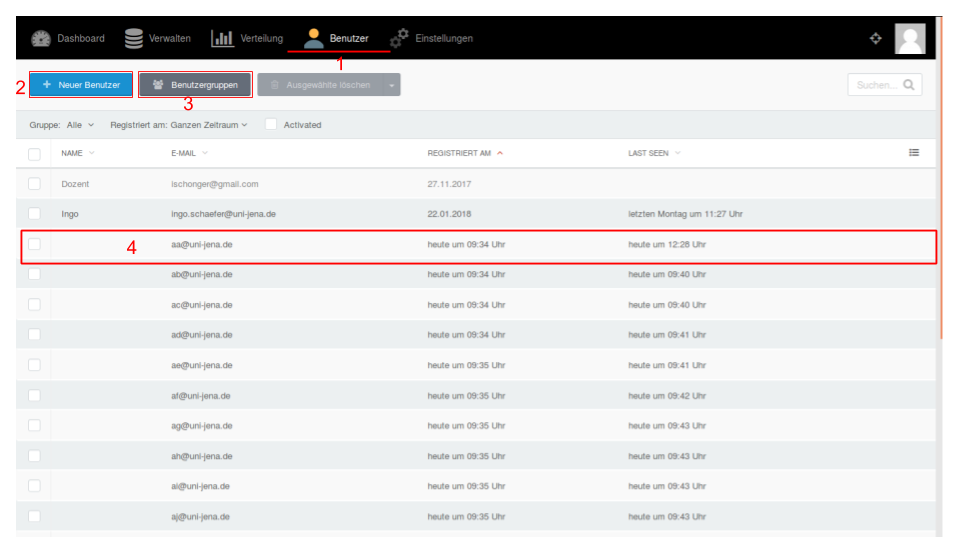
\includegraphics[scale=0.3]{backend/img/users_1.png}
  \begin{enumerate}
   \item In der Hauptnavigation gelangt der Nutzer durch den Punkt \textbf{Benutzer} in diese Übersicht.
	 Hier werden die registrierten Studenten aufgelistet.
   \item Soll ein weiterer Student hinzugefügt werden geschieht dies über den Button \textbf{+ Neuer Benutzer}.
	 Dann gelangt der Nutzer auf die Seite, die hier drunter abgebildet ist.
   \item Möchte der Nutzer die angemeldeten Studenten gruppieren. Geschieht dies über den Button \textbf{Benutzergruppen}.
   \item Durch Klicken auf eine der Zeilen, gelangt man auf eine Detailseite, welche den Studenten genauer aufführt.
	 Näheres in der dritten Abbildung in diesem Teilkapitel.
  \end{enumerate}

  
  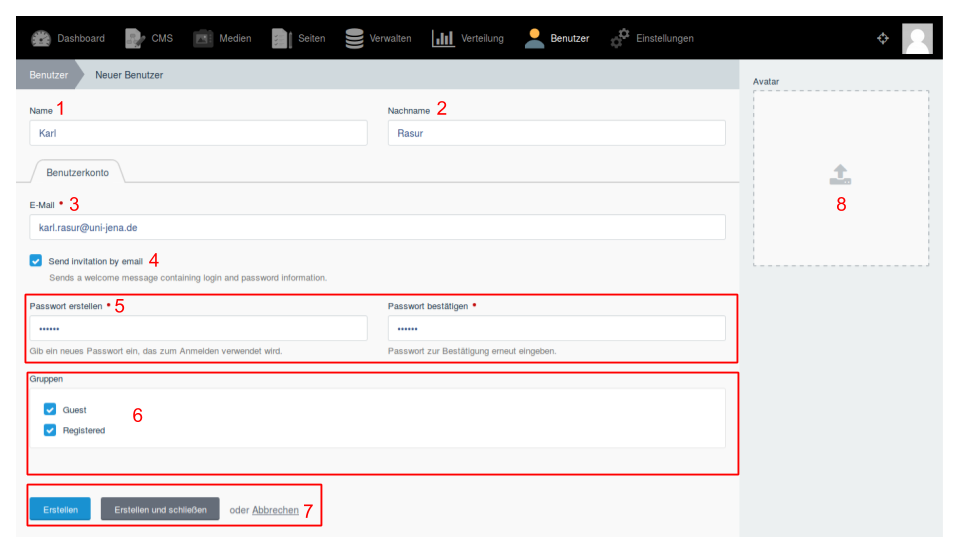
\includegraphics[scale=0.3]{backend/img/neuer_benutzer.png}
  \begin{enumerate}
   \item Hier kann ein Vorname eingegeben werden.
   \item Hier der Nachname.
   \item Einzige Pflichtangabe eines Studenten ist hier seine E-Mail. Dazu ist immer die Uni-Adresse (@uni-jena.de) zu verwenden.
   \item Indem hier der Haken gesetzt wird, wird eine E-Mail an die angegebene E-Mailadresse versendet, in der der Studierende dazu aufgefordert wird, sich auf der BWolf-Plattform anzumelden.
   \item In diesem Feld muss dem neuen Studenten ein vorläufiges Passwort übergeben werden.
   \item Wenn Gruppen angelegt wurden, kann der Nutzer hier dem neu angelegten Studenten in eine oder mehrere Gruppen zuweisen.
   \item Abschließend wird der Student angelegt, in dem der Nutzer auf einen der \textbf{Speichern}-Buttons klickt.
   \item Zusätzlich kann dem neuen Studenten hier über die Fläche \textbf{Avatar} ein Bild hinzugefügt werden.
  \end{enumerate}

  
  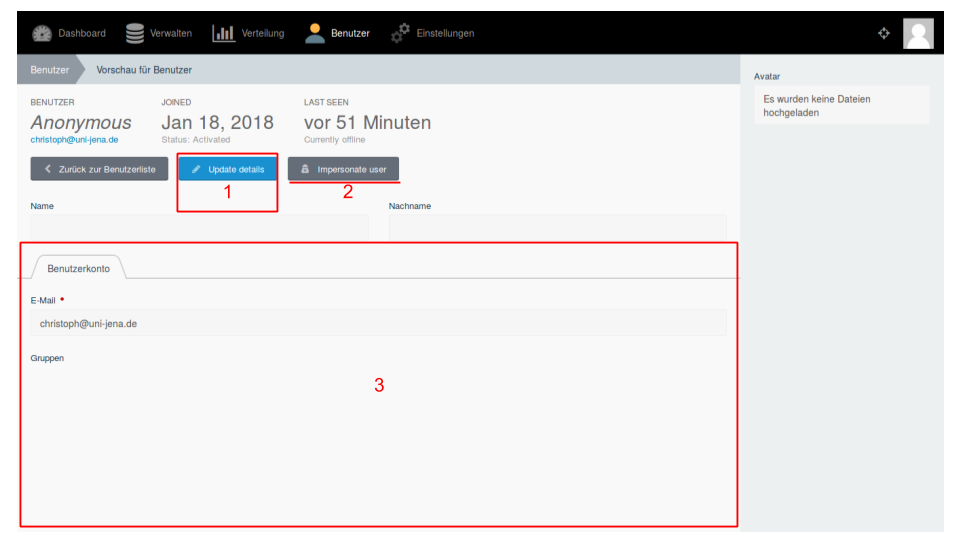
\includegraphics[scale=0.3]{backend/img/users_3.png}
  \begin{enumerate}
   \item neue Angaben können hier über den Button \textbf{Update details} übernommen werden
   \item Durch die Klickfläche \textbf{Impersonate user} kann der hier ausgewählte Nutzer entfernt werden.
   \item In diesen Eingabefeldern kann dem Studenten eine neue E-Mail und gegebenenfalls Gruppen zugewiesen werden.
  \end{enumerate}

  
  
  \section{Einstellungen}
  \label{section:settings}
  
  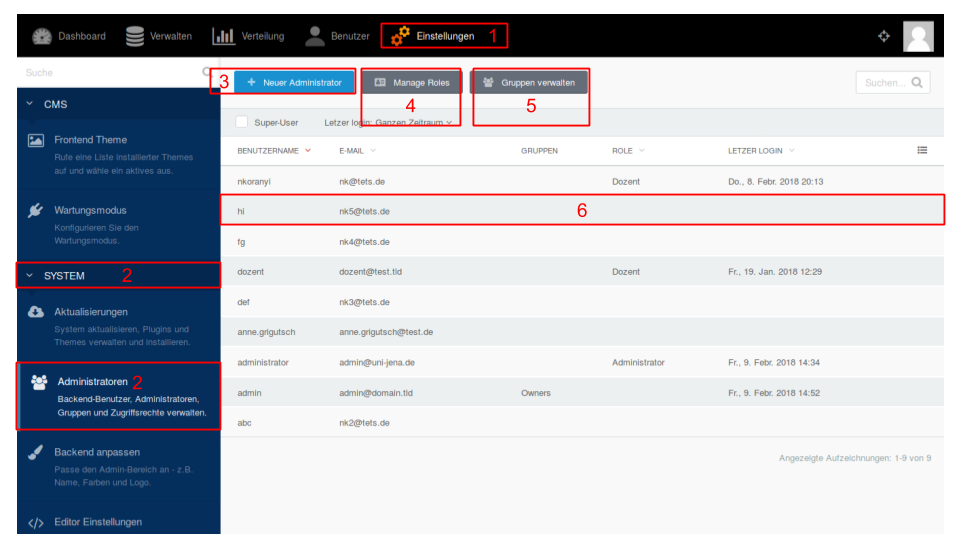
\includegraphics[scale=0.3]{backend/img/settings_1.png}
  \begin{enumerate}
   \item Über den Punkt \textbf{Einstellungen} kann der Nutzer in diese Ansicht wechseln.
	 Die zahlreichen Funktionen, die hier möglich sind, sind in der Regel für den operativen Normalbetrieb nicht anzupassen.
   \item Jedoch gelangt der Nutzer mithilfe des Punktes \textbf{Administratoren} unter \textbf{System} in der linken Vertikalnavigation in die hier aufgezeigte Ansicht.
   \item Dank des Buttons \textbf{+ Neuer Administrator} kann ein neuer angelegt werden. 
	 Dies geschieht analog zu der Weise, wie auch ein neuer Student in dem Menü Benutzer erstellt wird.
   \item[4. und 5.] Hier kann eine weitere Art von Nutzern eingestellt werden. Ist eigentlich nicht notwendig.
   \item[6.] Hier können die Einstellungen eines Nutzers angepasst werden. 
	 Die Ansicht dafür ist ähnlich wie die, in der Studenten verändert werden können.
  \end{enumerate}

    